\documentclass[twoside,10pt]{book}
\usepackage{graphicx}
\usepackage{hyperref}
\usepackage{xcolor}
\usepackage[utf8]{inputenc}
\usepackage{soul}

%----------------------------------------------------------------------------------------
%	MACROS
%----------------------------------------------------------------------------------------

\definecolor{menugray}{RGB}{230,230,230}
\sethlcolor{menugray} 
\newcommand{\menu}[1]{\hl{\texttt{#1}}}

%----------------------------------------------------------------------------------------
%	ENVIRONMENTS
%----------------------------------------------------------------------------------------

\definecolor{color-info}{RGB}{0,0,128} 
\newenvironment{info}{\begin{description}\item[\textcolor{color-info}{Information.}]}{\end{description}}

\definecolor{color-warning}{RGB}{128,0,0} 
\newenvironment{warning}{\begin{description}\item[\textcolor{color-warning}{Warning.}]}{\end{description}}

\newsavebox{\mybox}
\newenvironment{example}
{\begin{lrbox}{\mybox}\begin{minipage}{0.9\textwidth}}
{\end{minipage}\end{lrbox}\fbox{\usebox{\mybox}}}

%----------------------------------------------------------------------------------------
%	DOCUMENT INFO
%----------------------------------------------------------------------------------------

\title{Practical Systems Engineering}
\author{by the Systems Engineering Community}

%----------------------------------------------------------------------------------------
%	START DOCUMENT
%----------------------------------------------------------------------------------------

\begin{document}        

\maketitle

\tableofcontents

\chapter{Introduction}
Requirements Management and Engineering (RE\&M) is taught, both in industry and academia. The availability of open source SE-tools, and Eclipse-based tools in particular, created some interest for using those tools for teaching. 

As RE\&M is often seen as a discipline of Systems Engineering, our scope is systems engineering, with an \textbf{initial} focus on requirements engineering.

%===============================================================================
\section{Vision}
%===============================================================================

The vision of this project is to create:

\begin{enumerate}
\item A set of teaching materials that is actively used; 
\item Which is embedded in a larger SE context; and
\item Which explicitly focuses on applying RE. 
\end{enumerate}

%===============================================================================
\section{Scope}
%===============================================================================

The scope is the creation of teaching materials, centered around a case study, based on existing methods and tools. This is visualized in Figure~\ref{fig:scope}.

\begin{figure}[h!]
  \centering
  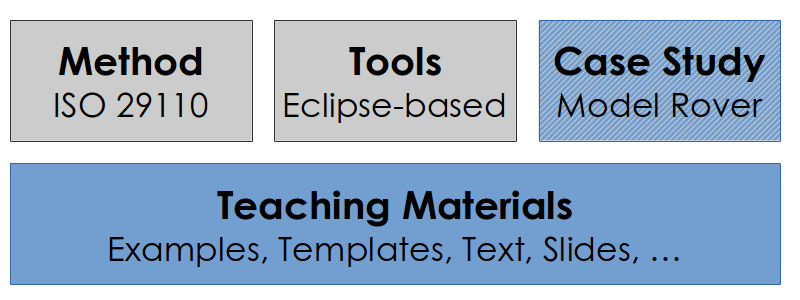
\includegraphics[width=\textwidth]{../se-images/teaching-overview.png}
  \caption{Scope of the SE teaching materials}
  \label{fig:scope}
\end{figure}

%-------------------------------------------------------------------------------
\subsection{Software vs. Systems Engineering}
%-------------------------------------------------------------------------------

For the purpose of this tutorial, a system has interfaces with other software or hardware, while software is (more or less) stand-alone.  Using this definition, we see systems engineering simply as an extension to software engineering, but with interfaces that can be unreliable.

%-------------------------------------------------------------------------------
\subsection{Standards}
%-------------------------------------------------------------------------------

ISO 29110 looks promising as the foundation for the method. Eclipse-based tools in general, and ProR for requirements engineering in particular, will be used. We are currently looking for a suitable case study, ideally using something that already exists. The focus will be on the creation of shared teaching materials. 
%-------------------------------------------------------------------------------

%===============================================================================
\section{Tools}
%===============================================================================

A central idea of this project is the use of freely available tools, as we cannot expect students to invest in expensive tools.  Tools will be based on Eclipse.  Figure~\ref{fig:v-model} shows on the left a simplified V-Model, depicting the tools we plan to use.

\begin{figure}[h!]
  \centering
  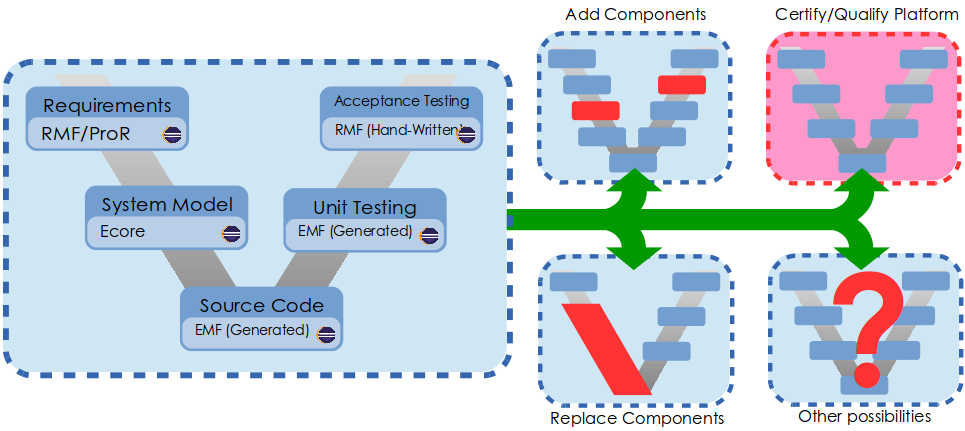
\includegraphics[width=\textwidth]{../se-images/toolchain.pdf}
  \caption{Tools used in this course}
  \label{fig:v-model}
\end{figure}

\begin{info}
In a ``real'' project, there would be many more tools and artifacts.  We will keep tools and artifacts to a minimum, in order not to overwhelm the students.
\end{info}

As you can see, we plan on building a \textbf{minimal, complete, Eclipse-based} software engineering platform.  It is loosely organized according to the V-Model.

%-------------------------------------------------------------------------------
\subsection{Modularity and Extendability}
%-------------------------------------------------------------------------------

Figure~\ref{fig:v-model} depicts on the right how this toolchain can be adapted to your needs.


Openness helps drastically to make this possible:

\begin{description}
\item[Open Standards] make it possible to replace individual tool components, without disturbing the toolchain as a whole.  Open Standards that we use include ReqIF, Java and JUnit.
\item[Open Software] allows the toolchain to be tailored and seamlessly integrated in a way that is very difficult to do otherwise.
\end{description}

%===============================================================================
\section{Background}
%===============================================================================

This project started in July 2014 as a discussion on \href{https://www.linkedin.com/groupItem?commentID=-1&item=5890782095432781827&type=member&gid=128312&view=}{LinkedIn}.  Thank you to all contributors!

%===============================================================================
\section{License}
%===============================================================================

This content is licensed as Apache 2.0.  If you contribute to the corresponding gitHub repository, you implicitly license the content that way.




\chapter{Case Study}
We have not decided on a case study yet.  Candidates so far are:

\begin{description}
\item[Coffee Maker.] A long-time favorite, and there are at least three available
\item[FAA Isolette.] This is a complete example from a safety-critical domain. 
\item[Rover.] This one is driven by Gaël Blondelle from the Eclipse Foundation. On the plus side, it's great for the classroom, as the hardware is cheap. But in contrast to the others, there is nothing there yet. 
\end{description}

Teaching Materials can be made available via \href{../se-materials/Example.reqif}{relative links}.


\end{document}

